% mnras_template.tex
%
% LaTeX template for creating an MNRAS paper
%
% v3.0 released 14 May 2015
% (version numbers match those of mnras.cls)
%
% Copyright (C) Royal Astronomical Society 2015
% Authors:
% Keith T. Smith (Royal Astronomical Society)

% Change log
%
% v3.0 May 2015
%    Renamed to match the new package name
%    Version number matches mnras.cls
%    A few minor tweaks to wording
% v1.0 September 2013
%    Beta testing only - never publicly released
%    First version: a simple (ish) template for creating an MNRAS paper

%%%%%%%%%%%%%%%%%%%%%%%%%%%%%%%%%%%%%%%%%%%%%%%%%%
% Basic setup. Most papers should leave these options alone.
\documentclass[a4paper,fleqn,usenatbib]{mnras}

% MNRAS is set in Times font. If you don't have this installed (most LaTeX
% installations will be fine) or prefer the old Computer Modern fonts, comment
% out the following line
\usepackage{newtxtext,newtxmath}
% Depending on your LaTeX fonts installation, you might get better results with one of these:
%\usepackage{mathptmx}
%\usepackage{txfonts}

% Use vector fonts, so it zooms properly in on-screen viewing software
% Don't change these lines unless you know what you are doing
\usepackage[T1]{fontenc}
\usepackage{ae,aecompl}


%%%%% AUTHORS - PLACE YOUR OWN PACKAGES HERE %%%%%

% Only include extra packages if you really need them. Common packages are:
\usepackage{graphicx}	% Including figure files
\usepackage{amsmath}	% Advanced maths commands
\usepackage{amssymb}	% Extra maths symbols

%%%%%%%%%%%%%%%%%%%%%%%%%%%%%%%%%%%%%%%%%%%%%%%%%%

%%%%% AUTHORS - PLACE YOUR OWN COMMANDS HERE %%%%%

% Please keep new commands to a minimum, and use \newcommand not \def to avoid
% overwriting existing commands. Example:
%\newcommand{\pcm}{\,cm$^{-2}$}	% per cm-squared

\newcommand{\Msun}{\mathrm{M_{\sun}}}

%%%%%%%%%%%%%%%%%%%%%%%%%%%%%%%%%%%%%%%%%%%%%%%%%%

%%%%%%%%%%%%%%%%%%% TITLE PAGE %%%%%%%%%%%%%%%%%%%

% Title of the paper, and the short title which is used in the headers.
% Keep the title short and informative.
\title[]{Insert clever, witty title here...}

% The list of authors, and the short list which is used in the headers.
% If you need two or more lines of authors, add an extra line using \newauthor
\author[I.D. Roberts \& L.C. Parker]{
Ian D. Roberts,\thanks{E-mail: roberid@mcmaster.ca}
Laura C. Parker
\\
% List of institutions
Department of Physics and Astronomy, McMaster University, Hamilton ON
L8S 4M1, Canada
}

% These dates will be filled out by the publisher
\date{Accepted XXX. Received YYY; in original form ZZZ}

% Enter the current year, for the copyright statements etc.
\pubyear{2016}

% Don't change these lines
\begin{document}
\label{firstpage}
\pagerange{\pageref{firstpage}--\pageref{lastpage}}
\maketitle

% Abstract of the paper
\begin{abstract}
\end{abstract}

% Select between one and six entries from the list of approved keywords.
% Don't make up new ones.
\begin{keywords}
galaxies: clusters: general -- galaxies: evolution -- galaxies:
groups: -- galaxies: statistics
\end{keywords}

%%%%%%%%%%%%%%%%%%%%%%%%%%%%%%%%%%%%%%%%%%%%%%%%%%

%%%%%%%%%%%%%%%%% BODY OF PAPER %%%%%%%%%%%%%%%%%%

\section{Introduction}
\label{sec:introduction}

%%%%%%%%%%%%%%%%%%%%%%%%%%%%%%%%%%%%%%%%

\section{Data}
\label{sec:data}

\subsection{Yang group catalogue}

\subsection{Field catalogue}

\subsection{Group dynamics}

\subsection{Matched data set}

\begin{figure*}
  \centering
  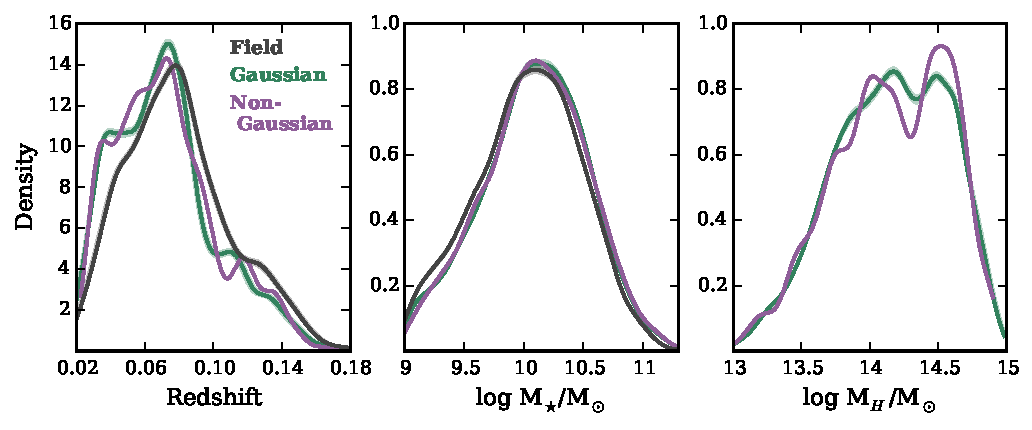
\includegraphics[width=\textwidth]{dist_m2_s.pdf}
  \caption{}
  \label{fig:dist_m2_s}
\end{figure*}

To ensure a fair comparison between galaxies in different environments
(ie.\ field galaxies, galaxies in G groups, and galaxies in NG groups)
we match our sample of G group galaxies and NG group galaxies by
stellar mass, redshift, and halo mass.  Additionally, we then match
our sample of field galaxies by stellar mass and redshift ensuring
that all of our galaxy samples are matched according to important galaxy
properties.  This is especially important when trying to elucidate
information on the effect of group dynamics on galaxy SF and
morphological properties for
two main reasons:
\par
First, stellar mass, redshift, and halo mass have
all been shown to influence galaxy SF and morphology (REF); whereas
the impact of group dynamics has been more difficult to pin down
(REF) which is perhaps suggestive of a more modest role.  Therefore,
if one hopes to identify trends in galaxy SF and morphology with group
dynamics it is crucial to properly control for these other effects.
\par
Second, standard statistical normality tests, such as the AD test, are
inherently biased in identifying non-Gaussian distributions when
sample size is large.  This is a result of the statistical power of
the test increasing with sample size which subsequently allows the
detection of more and more subtle departures from normality.  These subtle
departures from normality may not be physically relevant (in
principle, no group is truly Gaussian anyways) and what really matters is
whether galaxies in groups which show large departures from normality
have different properties than galaxies in groups which show smaller
departures from normality. Since group
richness tends scales with halo mass, in the absence of any matching
procedure, a sample of NG groups will be biased towards large halo
masses compared to a similar sample of G groups -- even though many
high halo mass NG groups may have been identified on the basis of very
small departures from normality.  Ensuring that our G and NG
samples have very similar halo mass distributions allows us to make a
fairer comparison between the two samples.

\begin{figure}
  \centering
  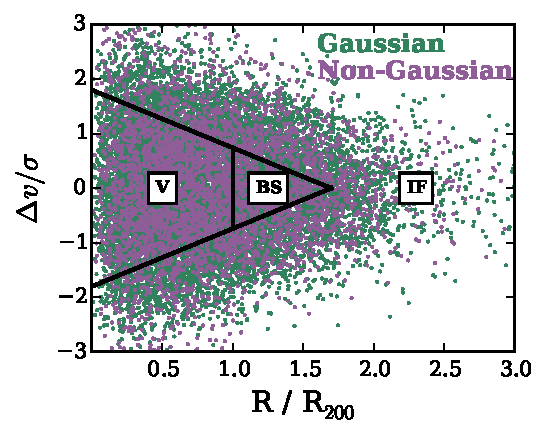
\includegraphics[width=\columnwidth]{vnorm_r.pdf}
  \caption{}
  \label{fig:vnorm_r}
\end{figure}

%%%%%%%%%%%%%%%%%%%%%%%%%%%%%%%%%%%%%%%%%%%%

\section{Results}
\label{sec:results}

\subsection{Infalling region}

\begin{figure*}
  \centering
  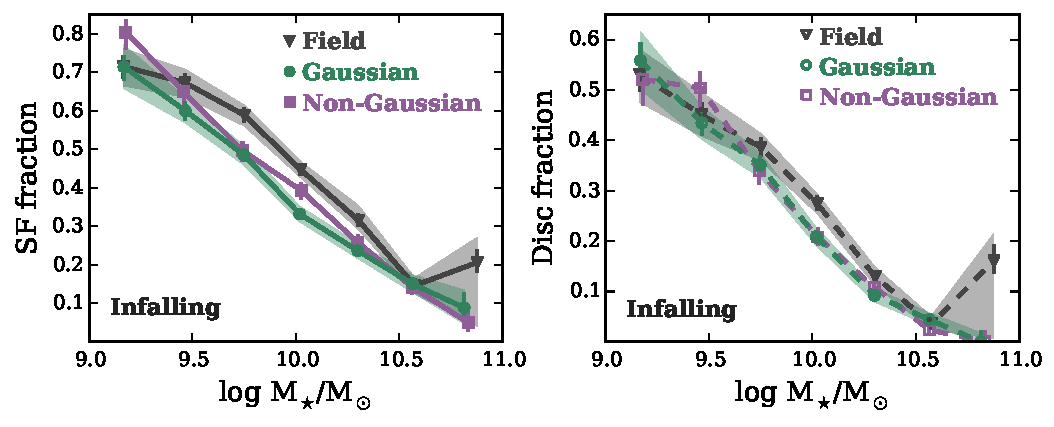
\includegraphics[width=\textwidth]{disk_sfFrac_w2_if.pdf}
  \caption{}
  \label{fig:disk_sfFrac_if}
\end{figure*}

\begin{figure}
  \centering
  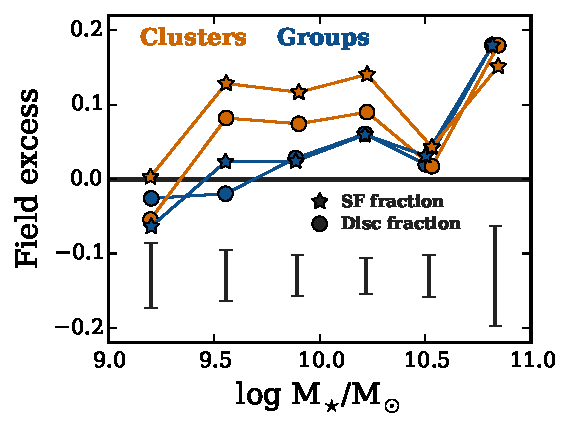
\includegraphics[width=\columnwidth]{mh_excess.pdf}
  \caption{}
  \label{fig:mh_excess}
\end{figure}

\subsection{Virialized region}

\begin{figure*}
  \centering
  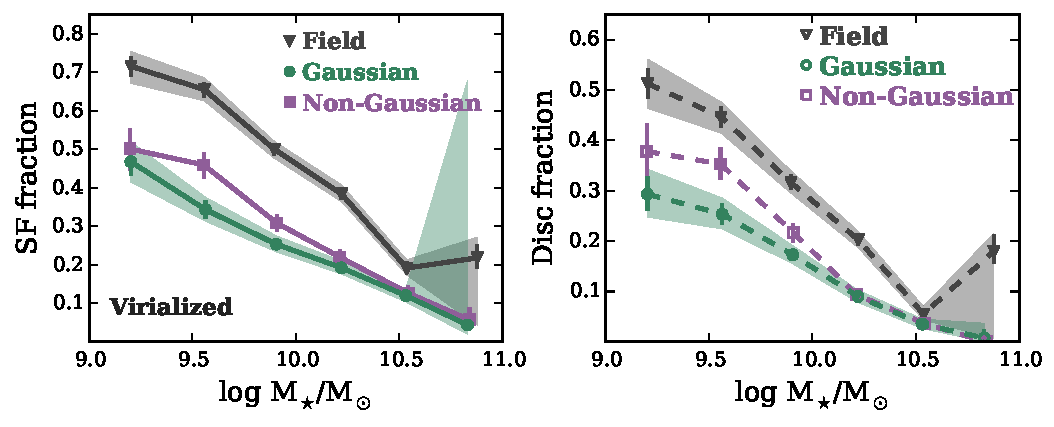
\includegraphics[width=\textwidth]{disk_sfFrac_w2_v.pdf}
  \caption{}
  \label{fig:disk_sfFrac_v}
\end{figure*}

%%%%%%%%%%%%%%%%%%%%%%%%%%%%%%%%%%%%%%%%%%%

\section{Discussion}
\label{sec:discussion}

%%%%%%%%%%%%%%%%%%%%%%%%%%%%%%%%%%%%%%%%%%%

\section{Summary \& conclusions}
\label{sec:summary} 

%%%%%%%%%%%%%%%%%%%%%%%%%%%%%%%%%%%%%%%%%%

\section*{Acknowledgments}
\label{sec:acknowledgments}

IDR thanks the Ontario Graduate Scholarship program for funding.  LCP
thanks the National Science and Engineering Research
Council of Canada for funding.  The authors thank
F. Evans for matching together the various SDSS catalogues used in
this research.  We thank X. Yang et al. for
making their
SDSS DR7 group catalogue publicly available, L. Simard et al. for the
publication of their SDSS DR7 morphology catalogue, J. Brinchmann et al. for
publication of their SDSS SFRs, and the NYU-VAGC
team for the 
publication of their SDSS DR7 catalogue.  This research would not have
been possible without access to these public catalogues.
\par
Funding for the SDSS has been provided by the Alfred P. Sloan
Foundation, the Participating Institutions, the National Science
Foundation, the U.S. Department of Energy, the National Aeronautics
and Space Administration, the Japanese Monbukagakusho, the Max Planck
Society, and the Higher Education Funding Council for England. The
SDSS Web Site is http://www.sdss.org/.
\par
The SDSS is managed by the Astrophysical Research Consortium for the
Participating Institutions. The Participating Institutions are the
American Museum of Natural History, Astrophysical Institute Potsdam,
University of Basel, University of Cambridge, Case Western Reserve
University, University of Chicago, Drexel University, Fermilab, the
Institute for Advanced Study, the Japan Participation Group, Johns
Hopkins University, the Joint Institute for Nuclear Astrophysics, the
Kavli Institute for Particle Astrophysics and Cosmology, the Korean
Scientist Group, the Chinese Academy of Sciences (LAMOST), Los Alamos
National Laboratory, the Max-Planck-Institute for Astronomy (MPIA),
the Max-Planck-Institute for Astrophysics (MPA), New Mexico State
University, Ohio State University, University of Pittsburgh,
University of Portsmouth, Princeton University, the United States
Naval Observatory, and the University of Washington.

%%%%%%%%%%%%%%%%%%%%%%%%%%%%%%%%%%%%%%%%%%%%%%%%%%

%%%%%%%%%%%%%%%%%%%% REFERENCES %%%%%%%%%%%%%%%%%%

% The best way to enter references is to use BibTeX:

\bibliographystyle{mnras}
\bibliography{RobertsParker2016} % if your bibtex file is called example.bib


% Alternatively you could enter them by hand, like this:
% This method is tedious and prone to error if you have lots of references
%\begin{thebibliography}{99}
%\bibitem[\protect\citeauthoryear{Author}{2012}]{Author2012}
%Author A.~N., 2013, Journal of Improbable Astronomy, 1, 1
%\bibitem[\protect\citeauthoryear{Others}{2013}]{Others2013}
%Others S., 2012, Journal of Interesting Stuff, 17, 198
%\end{thebibliography}


% Don't change these lines
\bsp	% typesetting comment
\label{lastpage}
\end{document}

% End of mnras_template.tex
